\section{Photo-$z$ performance}
\label{sec:photoz}

In this section we compute the photometric redshifts $z_{ph}$ of the galaxies in the Bright Sample (BS) and the Faint Sample (FS) generated in the previous section and analyze the performance of their photo-$z$ determination through different statistical metrics: bias, photo-$z$ precision and outlier fraction. We also apply some photo-$z$ quality cuts (\textit{odds} cuts) on the results and analyze how the performance improves. We investigate how many galaxies with poor photo-$z$ quality we need to remove in order to achieve the photo-$z$ precision requirements defined in \citet{Gaztanaga2012}.

The photo-$z$s $z_{ph}$ are obtained using the Bayesian Photometric Redshifts\footnote{\texttt{BPZ} can be found at \url{http://www.its.caltech.edu/~coe/BPZ/}.} (BPZ) template-fitting code described in~\citet{Benitez2000}. It uses Bayesian statistics to produce a posterior probability density function $p(z|m_j)$ that a galaxy is at redshift $z$ when its magnitudes in the different bands $j$ are $m_j$:
\begin{equation}
p(z|m_j) \propto \sum_t L(m_j|z,t) \, \Pi(z,t \mid m)  \, ,
\label{pz}
\end{equation}
where $L(m_j|z,t)$ is the likelihood that the galaxy has magnitudes $m_j$, if its redshift is $z$ and its spectral type $t$, and $\Pi(z,t \mid m)$ is the prior probability that the galaxy has redshift $z$ and spectral type $t$ when its magnitude in some reference band is $m$. The proportionality symbol is a reminder that $p(z|m_j)$ must be properly normalized in order to be a probability density function. The photometric redshift $z_{ph}$ of the galaxy will be taken as the position of the maximum of $p(z|m_j)$.

We have modified the {\tt BPZ} code in order to increase its efficiency when estimating photo-$z$s using a large number of narrow-band filters. Instead of estimating the
photo-$z$ for each galaxy, the calculations are done in blocks
of hundreds of galaxies using linear operations. Details will
be presented in Eriksen et al.~(in preparation).

\subsection{Templates}
The likelihood $L(m_j|z,t)$ is generated by comparing the observed magnitudes with the ones that are predicted through a collection of galaxy templates that span all possible galaxy types $t$. BPZ includes its own template library; however, we use a subset of 6 templates from the same library used in the previous section for the mock catalog generation. They are highlighted in Fig.~\ref{pau_templates} and correspond to the templates with file name: \texttt{CWW\_Ell.sed}, \texttt{Ell\_09.sed}, \texttt{CWW\_Sbc.sed}, \texttt{CWW\_Scd.sed}, \texttt{CWW\_Irr.sed} and \texttt{I99\_05Gy.sed}. Additionally, we also include two interpolated templates between each consecutive pair of the six by setting the \texttt{BPZ} input parameter \texttt{INTERP=2}. This results in a total of 16 templates. However, we will see later in Fig.~\ref{dz_hist_bright} that the number of interpolated templates does not affect much the photo-$z$ performance.

\subsection{Prior}
An important point of \texttt{BPZ} is the prior probability $\Pi(z, t \mid m)$ that helps improve the photo-$z$ performance. \citet{Benitez2000} proposes the following empirical function:
\begin{eqnarray}
\Pi(z, t \mid m) &=& \Pi(t\mid m) \cdot \Pi(z \mid t, m) \nonumber \\
&\propto& f_t e^{-k_t(m-m_0)} \cdot z^{\alpha_t}\exp \left\lbrace -\left[ {z \over z_{mt}(m)} \right]^{\alpha_t} \right\rbrace \nonumber \\
\label{prior_pau}
\end{eqnarray}
where $z_{mt}(m) = z_{0t} + k_{mt}(m-m_0)$ and $m_0$ is a reference magnitude, in our case equal to 19 in the $i$-band. Each spectral type $t$ has associated a set of five parameters $\lbrace f,k,\alpha,z_0,k_{m} \rbrace$ that determine the shape of the prior. In order to calibrate the prior $\Pi(z,t\mid m)$ and determine the value of these parameters, we construct a training sample consisting of 10000 galaxies randomly selected from the mock catalog with $i_{AB}<24$. We only need to know their observed magnitude $i_{AB}$ in our reference band, their true redshift $z_{tr}$ and their true spectral type $t_{tr}$. Originally, $t$ ranged from 0 to 66 which is the number of templates used to generate the mock catalog; however, as we did for the Luminosity Functions (LF) galaxy types in the previous section, we group all these galaxy types in three groups: $t=1$ (ellipticals), $t=2$ (spirals) and $t=3$ (irregulars), whose correspondence is 1$\rightarrow$(0-17), 2$\rightarrow$(17-55) and 2$\rightarrow$(55-66). From now on, we will use $t$ for either the 66 templates or these 3 galaxy type groups. Finally, we fit Eq.~(\ref{prior_pau}) to the training sample and recover the prior parameters. We show the resulting values in Table~\ref{tab:prior_pau}. Parameters $f_3$ and $k_3$ do not appear in the table because $\Pi(t=3 \mid m_0)$ is deduced by imposing the proper normalization.
\begin{table}
\centering
\begin{tabular}{cccccc}
\hline
$t$ & $f$ & $k$ & $\alpha$ & $z_0$ & $k_{m}$ \\ \hline
1&0.565&0.186&2.456&0.312&0.122\\
2&0.430&0.000&1.877&0.184&0.130\\
3&-&-&1.404&0.047&0.148\\
\hline
\end{tabular}
\caption{The resulting values of the prior parameters obtained by fitting (\ref{prior}) to a subset of 10000 randomly selected galaxies from the BS and FS together. The three galaxy types $t=1,2,3$ are the same that were defined in Section~\ref{sec:mock} for the Luminosity Functions (LF). $f_3$ and $k_3$ do not appear because $\Pi(t=3 \mid m_0)$ is deduced by normalization.}
\label{tab:prior_pau}
\end{table}
\begin{figure*}
\centering
\begin{tabular}{rl}
\includegraphics[height=100mm]{./plots/pau_t_prior_plot.pdf} & \includegraphics[height=100mm]{./plots/pau_z_prior_plot.pdf} 
\end{tabular}
\caption{Left: Comparison between the fitted $\Pi(t|m)$ prior (red) of Eq.~(\ref{prior}) and the actual distribution (black). Right: The same for $\Pi(z|t,m)$. We only differentiate between 3 galaxy types $t$ (as we did for the LFs in section~\ref{sec:mock}): 1 = Elliptical, 2 = Spiral and 3 = Irregular. Rows correspond to $i_{AB}$ magnitude bins of width $\Delta m=0.2$ centered at values from $m=19$ to $24$ in steps of $1$. All curves have been normalized. Resulting prior parameters are on Table~\ref{tab:prior}.}
\label{pau_prior_plot}
\end{figure*}
In Fig.~\ref{pau_prior_plot}, we show a comparison between the fitted curve and the actual distribution of the prior. $\Pi(t|m)$ on the left and $\Pi(z|t,m)$ on the right  are shown at different magnitudes (rows) from $i_{AB}=19$, the reference magnitude, to $i_{AB}=24$. On the one hand, the fitted $\Pi(t|m)$ agrees by definition with the actual distribution at the reference magnitude (top row), since we use those values as a starting point. However, at higher magnitudes a significant mismatch appears for the spiral and irregular galaxies. This is related to the fact that the $k$ parameters, which control the migration of galaxies from one spectral type to another across magnitude, are positive definite. With this, elliptical and spiral galaxies should turn to Irregulars as the magnitude increases. However, in Fig.~\ref{pau_prior_plot} we observe that actually the spiral abundance grows slightly before starting to decrease at $m\sim21$, and this forces the fit to $k_2=0$. Consequently, elliptical galaxies migrate directly to irregulars, causing a mismatch on the pace of growth of this galaxy type abundance. On the other hand, the fit of $\Pi(z|t,m)$ is particularly good for Ell and Sp galaxies at higher magnitudes (the eight bottom-left panels on the right plot of Fig.~\ref{pau_prior_plot}), but for Irr and magnitudes close to the 19 (the reference magnitude) it is less accurate.
\begin{figure}
\centering
\includegraphics[width=84mm]{./plots/Nz_pau.pdf}
\caption{Comparison between the true redshift (solid) and the photo-$z$ (discontinuous) distributions for the BS (red) and FS (blue). For the sake of clarity, we have set the \texttt{x}- and \texttt{y}-axis scales to be linear below the black dashed lines and logarithmic above them. All distributions have been normalized to equal area. Dashed lines correspond to the $z_{ph}$ obtained by maximizing only the likelihood $L(m_j|z,t)$ (ML) of (\ref{pz}), the dash-dotted line includes the prior (ML$\Pi$), and the dotted line corresponds to the case when all the $p(z|m_j)$ are stacked (pdf L$\Pi$).}
\label{z_hist}
\end{figure}
\begin{figure}
\centering
\includegraphics[width=84mm]{./plots/Dz_pau.pdf}
\caption{$\Delta z / (1+z_{tr})$ distributions, where $\Delta z \equiv z_{ph} - z_{tr}$, for the BS (red) and FS (blue) with the $z_{ph}$ obtained by maximizing only the likelihood $L(m_j|z,t)$ (ML) (solid) or when also including the prior (ML$\Pi$) (dotted). Photo-$z$ precision $\sigma_z$ values, defined as half of the symmetric interval that encloses the 68\% of the distribution area around the maximum, are shown for each case in the legend. The \texttt{x}-axis scale is linear between the two dashed vertical lines and logarithmic on the sides. Similarly, the \texttt{y}-axis is linear below the horizontal dashed line and logarithmic above. The prior makes no difference on the BS, but in the FS it removes the long tail (blue region) of catastrophic outliers ($|\Delta z|/(1+z_{tr})>1$) that accounts for a $\sim 7.7\%$ of the sample. This reduces $\sigma_z$ by a factor of $\sim$1.8.}
\label{dz_hist}
\end{figure}

In Fig.~\ref{z_hist} we show a comparison between the $z_{tr}$ (solid) and $z_{ph}$ (discontinuous) distributions for the BS and the FS. For the sake of clarity, the \texttt{x}- and \texttt{y}-axes have been set to be linear below $z=2$ and $N=0.1$ respectively, and logarithmic elsewhere. Dashed lines correspond to $z_{ph}$ obtained by maximizing only the likelihood $L(m_j|z,t)$ in (\ref{pz}). This gives a $z_{ph}$ distribution in the BS very close to the actual, while in the FS a residual long tail towards much higher redshift ($z\sim5$) appears. In Fig.~\ref{dz_hist} we show the equivalent $\Delta z / (1+z_{tr})$ distributions, where $ \Delta z \equiv z_{ph} - z_{tr}$. Once again, the \texttt{x}- and \texttt{y}-axes have been set to be linear below $|\Delta z| / (1+z_{tr})=1$ and $N=0.05$ respectively, and logarithmic elsewhere. Note that the tail is also present on the right-hand side of the blue curve. If we define as \textit{catastrophic outliers} those galaxies with $|\Delta z| / (1+z_{tr}) > 1$, we find that they account for $\sim$7.7\% in the FS (the blue region under the curve) and $\sim$0.2\% in the BS. Catastrophic outliers are typically caused by degeneracies in color space, which cause confusions in the template fit and result in a much larger $|\Delta z|$. The blue-dotted line in Fig.~\ref{dz_hist} shows that when the prior is included almost all of the catastrophic outliers in the FS are removed, leaving only a small fraction of $\sim0.1\%$. In fact, we see in Fig.~\ref{z_hist} that the $z_{ph}$ distribution after applying the prior (blue dot-dashed) decays at high redshifts faster than the $z_{tr}$ distribution. This is because we are only using the maximum of $p(z|m_j)$ for the $z_{ph}$ value. If we use the whole pdf information (blue-dotted line), the resulting $z_{ph}$ distribution is much closer to the true. Defining the photo-$z$ precision $\sigma_z$ as half of the symmetric interval that encloses the 68\% of the $\Delta z /(1+z_{tr})$ distribution area around the maximum, we find that $\sigma_z$ almost does not change in the BS (0.72\% to 0.70\%), while it improves by a factor $\sim1.8$ in the FS by going from $\sigma_z\sim16\%$ to $\sim8.86\%$ when adding the prior. 

\begin{figure}
\centering
\includegraphics[width=84mm]{./plots/Dz_pau_bright.pdf}
\caption{The $\Delta z / (1+z_{tr})$ distributions for the BS using different number of interpolated templates in \texttt{BPZ}, when input magnitudes are noiseless (solid) and when they are noisy (dotted). Photo-$z$ precision $\sigma_z$ values for each case are shown on the legend. The \texttt{x}-axis scale is linear between the two dashed vertical lines and logarithmic on the sides. Similarly, the \texttt{y}-axis is linear below the horizontal dashed line and logarithmic above.}
\label{dz_hist_bright}
\end{figure}

\subsection{Performance vs. template interpolation}
At this point, we want to explore how the number of interpolated templates used in \texttt{BPZ} changes the $z_{ph}$ performance. In Fig.~\ref{dz_hist_bright} we show the $\Delta z / (1+z_{tr})$ distribution only for the BS when we use: 9 (blue), 2 (red) and 0 (green), interpolated templates. Solid lines correspond to the $z_{ph}$ obtained when the input magnitudes are noiseless (without applying Eq.~\ref{noiselesstonoisy}), while dotted lines include the noise. The $\sigma_z$ of each distribution is shown in the legend. We see that, while for noiseless magnitudes the number of interpolated templates has a significant impact on the width of the distributions and so, on their $\sigma_z$, which gets worse by a factor of $\sim3$ at each step, for noisy magnitudes these differences are smaller. In fact, going from 9 to 2 interpolated templates the differences are negligibly small and going from 2 to 0 interpolations the difference is less than a factor of 2. 
%It is interesting to note that the shape and width of the distribution with no interpolations for the noiseless case (green-solid) is very similar to the shape of the distributions for the noisy case (dotted).
\begin{figure*}
\centering
\begin{tabular}{rl}
\includegraphics[type=pdf,ext=.pdf,read=.pdf, height=120mm]{./plots/mock.r260.n1e6.s10.121027_default_bright_interp2_whole} & \includegraphics[type=pdf,ext=.pdf,read=.pdf, height=120mm]{./plots/mock.r260.n1e6.s10.121027_default_faint_interp2_whole}
\end{tabular}
\caption{Top: $\Delta z/(1+z_{tr})$ distributions for the BS (left) and the FS (right) at different photo-$z$ quality cuts whose completeness, shown in a color degradation, range from 100\% (bluest) to 5\% (reddest) in 5\% steps. On the bottom and by rows: the bias (median), the photo-$z$ precision ($\sigma_z$) and the $3\sigma$-outlier fraction of the distributions at the top as a function of the completeness. The colors of the points match the colors in the distributions. Note that the vertical scale in the bias and the $\sigma_z$ panels changes by an order of magnitude between the two samples. The black-dashed horizontal lines on the $\sigma_z$ panels show the photo-$z$ precision requirements defined in \citet{Gaztanaga2012}: $\sigma_z<0.35\%$ (BS) and $<5\%$ (FS).}
\label{pz_results}
\end{figure*}

\subsection{Performance vs. \textit{Odds}}
Photo-$z$ codes, besides returning a best estimate for the redshift, typically also return an indicator of the photo-$z$ quality. It can be simply an estimation of the error on $z_{ph}$, or something more complex, but the aim is the same. In \texttt{BPZ} this indicator is called \textit{odds}, and, it is defined as
\begin{equation}
odds = \int^{z_{ph}+\delta z}_{z_{ph}-\delta z}p(z|m_j)dz \, ,
\label{odds}
\end{equation}
where $\delta z$ determines the redshift interval where the integral is computed. \textit{Odds} can range from 0 to 1, and the closer to 1, the more reliable is the photo-$z$ determination, since $p(z|m_j)$ becomes sharper and most of its area is enclosed within $z_{ph}\pm \delta z$. We choose $\delta z=$ 0.0035 in the BS and 0.05 in the FS, which is close to the expected $\sigma_z$ in these samples for the PAU Survey (see the $\sigma_z$ plots in Fig.~\ref{pz_results}). A bad choice of $\delta z$ could lead to the accumulation of all \textit{odds} close to either 0 or 1. Since \textit{odds} are a proxy for the photo-$z$ quality, we should expect a correlation between the \textit{odds} and $|\Delta z|$ in the sense that higher \textit{odds} should correspond to lower $|\Delta z|$. 

At the top of Fig.~\ref{pz_results}, we show the $\Delta z/(1+z_{tr})$ distributions in a color degradation for subsets of the BS (left) and the FS (right) with increasingly higher cuts on the \textit{odds} parameter. In fact, the exact \textit{odds} values are quite arbitrary, since they depend on the size of $\delta z$. Therefore, we have translated these \textit{odds} cuts into the fraction of the galaxy sample remaining after a certain cut has been applied, in such a way that the bluest curve corresponds to 100\% completeness while the reddest corresponds to 5\% completeness, with 5\% steps. We can clearly see how the harder are the \textit{odds} cuts, the narrower and peaky become the distributions in both samples. On the bottom plots of the same figure we show how some statistical metrics of these distributions (the bias (median), the photo-$z$ precision ($\sigma_z$) and the $3\sigma$-outlier fraction) evolve with each \textit{odds} cut of completeness given in the \texttt{x}-axis. The $3\sigma$-outlier fraction is defined as the fraction of galaxies with $|\Delta z|/(1+z_{tr})>3\sigma_z$. For the sake of clarity, each point has been colored as its corresponding distribution. Errors are computed by bootstrap \citep{efron79} for the bias and $\sigma_z$, and by computing the $\sigma_{68}$ of a binomial distribution with mean $n_{outlier} / N$ for the outlier fraction. As we expected, $\sigma_z$ decreases as the \textit{odds} cuts get more stringent. In the BS (left), it goes from $\sim$0.7\% at 100\% of completeness to $\sim$0.1\% at 5\%, and in the FS (right), from $\sim$9\% to $\sim$1\%. The photo-$z$ precision requirements, as defined in \citet{Gaztanaga2012}, are $\sigma_z < 0.35\%$ in the BS and $\sigma_z < 5\%$ in the FS. They are fulfilled when $\sim$50\% of each catalog is removed. We find a very small bias of a few percent of $\sigma_z$ in both samples towards negative $\Delta z$ values. It practically vanishes when high \textit{odds} cuts are applied. The $3\sigma$-outlier fraction in the BS starts at $\sim$13\%, drops to $\sim$3\% at $\sim$40\% completeness and then, starts increasing again up to $\sim$4.5\% at $\sim$10\% completeness. Therefore, we deduce that the gain on $\sigma_z$ with the \textit{odds} cut occurs basically through the cleaning of outliers. However, in the FS, even if $\sigma_z$ decreases with the \textit{odds} cuts, the outlier fraction increases from $\sim$7\% to $\sim$9\% at $\sim$15\% completeness. 
%Note that the outlier fraction drops sharply in both catalogs at lower completeness.

On the last three rows of plots in Figs.~\ref{bs_pz_results} (BS) and~\ref{fs_pz_results} (FS), we show how these statistical metrics evolve with the $i_{AB}$ observed magnitude (left), the true spectral type $t_{tr}$ (center) and the true redshift $z_{tr}$ (right), after each photo-$z$ quality cut shown in Fig.~\ref{pz_results} in the same color. In the top three rows and by order, we also show the scatter plot $\Delta z / (1+z_{tr})$, the number of galaxies and the completeness after the same photo-$z$ quality cuts with respect to the same variables ($i_{AB}$, $t_{tr}$,$z_{tr}$) on the \texttt{x}-axis.

In the BS (Fig.~\ref{bs_pz_results}), we can see that the low photo-$z$ quality galaxies (blue points in the scatter plot) are mostly faint galaxies with $i_{AB}>21$, the magnitude where the noise coming from the sky brightness plus the CCD read-out starts to be comparable to the Poisson noise in the signal. This is reflected in Fig.~\ref{err_m} as a turning point on the slope of the $\sigma_m$ vs. $m_{AB}$ scatter. In fact, these galaxies represent most of the outliers and the principal source of bias seen in Fig.~\ref{pz_results}. As the \textit{odds} cuts are applied, these bad photo-$z$ faint galaxies are removed. The \textit{odds} cut removes the bias, reduces $\sigma_z$ from $\sim$2.2\% to $\sim$0.35\% and the outlier fraction from $>$10\% to $\sim$1\% at magnitudes close to the limit $i_{AB}=22.5$. Looking at the scatter plots in the next two columns in Fig.~\ref{bs_pz_results}, we realize that these low-\textit{odds} galaxies at faint magnitude are spread out over the whole $t_{tr}$ and $z_{tr}$ ranges. Moreover, after the hardest \textit{odds} cut, only galaxies of types $t\sim0$ (elliptical) and $t\sim50$ (irregular) survive and the mean of $z_{tr}$ is shifted from $\sim$0.6 to $\sim$0.4. The worst bias, $\sigma_z$ and outlier fraction are obtained for Spiral galaxies ($t\sim$10-30). The \textit{odds} cuts mitigate these results, but even after applying them, spiral galaxies still have the worst bias and $\sigma_z$. The worst bias is located at low and high $z_{tr}$, with opposite sign and it is largely reduced with the \textit{odds} cuts. The value of $\sigma_z$ gets flatter over all $z_{tr}$ as the \textit{odds} cut gets harder.

Regarding the $z_{ph}$ precision requirement $\sigma_z < 0.35\%$ (black solid horizontal line), we find that, when no \textit{odds} cut is applied, it is achieved only for galaxies with $i_{AB}<21$ and galaxy type around $t\sim50$ (irregulars). However, it is not fulfilled at any $z_{tr}$. Once we apply a 50\% completeness \textit{odds} cut, which gives an overall $\sigma_z$ equal to the requirement, as we saw in Fig.~\ref{pz_results}, the requirement is fulfilled in all the $i_{AB}$ and $z_{tr}$ ranges. Only for spiral galaxies the requirement is not fulfilled even after the hardest \textit{odds} cut. Originally, in \citet{Benitez2009}, it was assumed that elliptical galaxies (or rather Luminous Red Galaxies) would yield the best photo-$z$ precision in the PAU Survey, with the narrow bands tracking the $\sim$4000\AA \ break spectral feature (Fig.~\ref{pau_templates}). This is partially true, since we actually see that elliptical galaxies give better $\sigma_z$ than spirals, but our analysis shows that in fact irregulars with $t\sim50$ give the best photo-$z$ performance. Before any \textit{odds} cut, their photo-$z$ precision is almost twice as better than the requirement. Probably this is due to the fact that, in contrast to elliptical galaxies were a single spectral feature is tracked, irregulars have the two emission lines [OII] $\sim$3737\AA \ and [OIII] $\sim$5000\AA \ (Fig.~\ref{pau_templates}) with intrinsic widths narrower than the width of the NB filters.
%{Due to the fact that the spectral template resolution in wavelenght is intended for broad bands in the photo-$z$ determination, these emision lines are still too coarse for the PAU narrow bands. A higher spectral resolution would probably improve the performance even more. On the other hand, the strength of these two lines is spuriously similar. In the real world these kind of lines whould have different heights what would result in a worse photo-$z$ performance. Therefore, simulations with different spectral line intensities and a higher template resolution would be needed to quanify the net effect of these opposing facts, but this is beyond the scope of this paper.}

\begin{figure*}
%\includegraphics[type=pdf,ext=.pdf,read=.pdf, width=130mm]{./plots/mock.r260.n1e6.s10.121027_default_bright_interp2}
\includegraphics[type=jpg,ext=.jpg,read=.jpg, width=130mm]{./plots/mock.r260.n1e6.s10.121027_default_bright_interp2}
\caption{Statistics showing the PAU-BS photo-$z$ performance as a function of the observed $i_{AB}$ magnitude (left), true galaxy type $t_{tr}$ (center) and true redshift $z_{tr}$ (right). In the first row we show the scatter $\Delta z/(1+z_{tr})$. Then, in a descending order of rows, we show the number of galaxies, the completeness, the bias (median), the photo-$z$ precision ($\sigma_z$) and the $3\sigma$-outlier fraction for all the \textit{odds} cuts shown in Fig.~\ref{pz_results} (same color). Also as in Fig.~\ref{pz_results}, the black-solid horizontal lines on the $\sigma_z$ panels show the photo-$z$ precision requirement defined in \citet{Gaztanaga2012}.}
\label{bs_pz_results}
\end{figure*}

In the FS (Fig.~\ref{fs_pz_results}), we see that the scatter of $\Delta z/(1+z_{tr})$ is much larger, as expected from the wider histograms in Fig.~\ref{pz_results}. However, a wider but still tight core close to $\Delta z = 0$ with high photo-$z$ quality (red points) remains. We recognize behaviors similar to those in the BS in most aspects of the $z_{ph}$ performance, although they are substantially larger. For example, the highest magnitude as well as lowest and highest $z_{tr}$ galaxies are the most biased. The \textit{odds} cuts also mitigate this bias, but a residual bias of opposite sign persists at the extremes of $z_{tr}$. Spiral galaxies ($t\sim10$-$30$) are also the ones with the highest bias, and the \textit{odds} cuts even aggravates this. We also see that elliptical ($t\sim0$) and irregular ($t>50$) galaxies are initially biased, but, in contrast to spirals, the \textit{odds} cuts help to reduce the bias. Unlike in the BS, $\sigma_z$ increases along all the magnitude range since at those magnitudes the noise from the sky brightness dominates over the signal (Fig.~\ref{err_m}). However, we see that the slope of the $\sigma_z$ increase is smaller the harder the \textit{odds} cuts. This is because the gain in photo-$z$ precision is at the expense of keeping only brighter galaxies each time. The mean $i_{AB}$ magnitude goes from $\sim$23.2 to $\sim$22.8 with the \textit{odds} cuts, and the shift in the $z_{tr}$ mean is from $\sim$0.86 to $\sim$0.81. Unlike in the BS, we see that the best $\sigma_z$ is obtained at the extremal spectral types: $t\sim0$ (elliptical) and $t\sim66$ (irregular). However, once the hardest \textit{odds} cuts are applied, irregular galaxies with $t\sim$50 are again the ones with the best $\sigma_z$. In fact, the hardest \textit{odds} cuts also remove all spiral galaxies. Note that the large bias seen at the extremes of $z_{tr}$ make $\sigma_z$ take values much larger at these redshifts. The photo-$z$ precision requirement, $\sigma_z<5\%$, is fulfilled when the \textit{odds} cut of 50\% completeness is applied up to magnitude $\sim23.1$, for all galaxy types except spirals, and at the $z_{tr}$ interval from $\sim0.4$ to $\sim1.3$. As we already saw on Fig.~\ref{pz_results}, the $3\sigma$-outlier fraction grows with the \textit{odds} cuts. In general, its values are higher where $\sigma_z$ is lower, since the outliers criterion becomes more stringent.
\begin{figure*}
%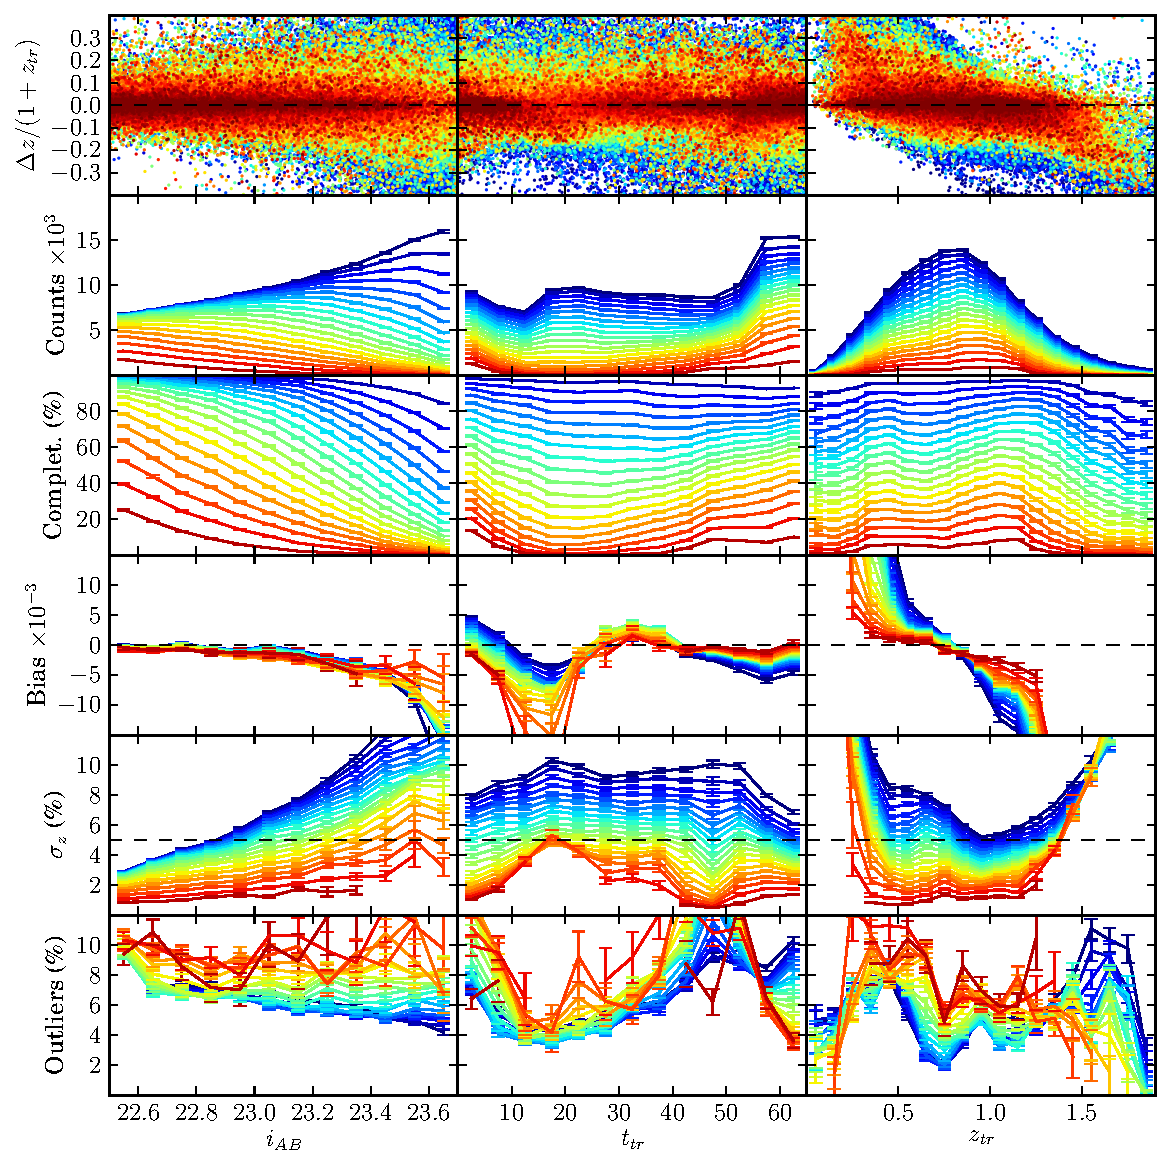
\includegraphics[type=pdf,ext=.pdf,read=.pdf, width=130mm]{./plots/mock.r260.n1e6.s10.121027_default_faint}
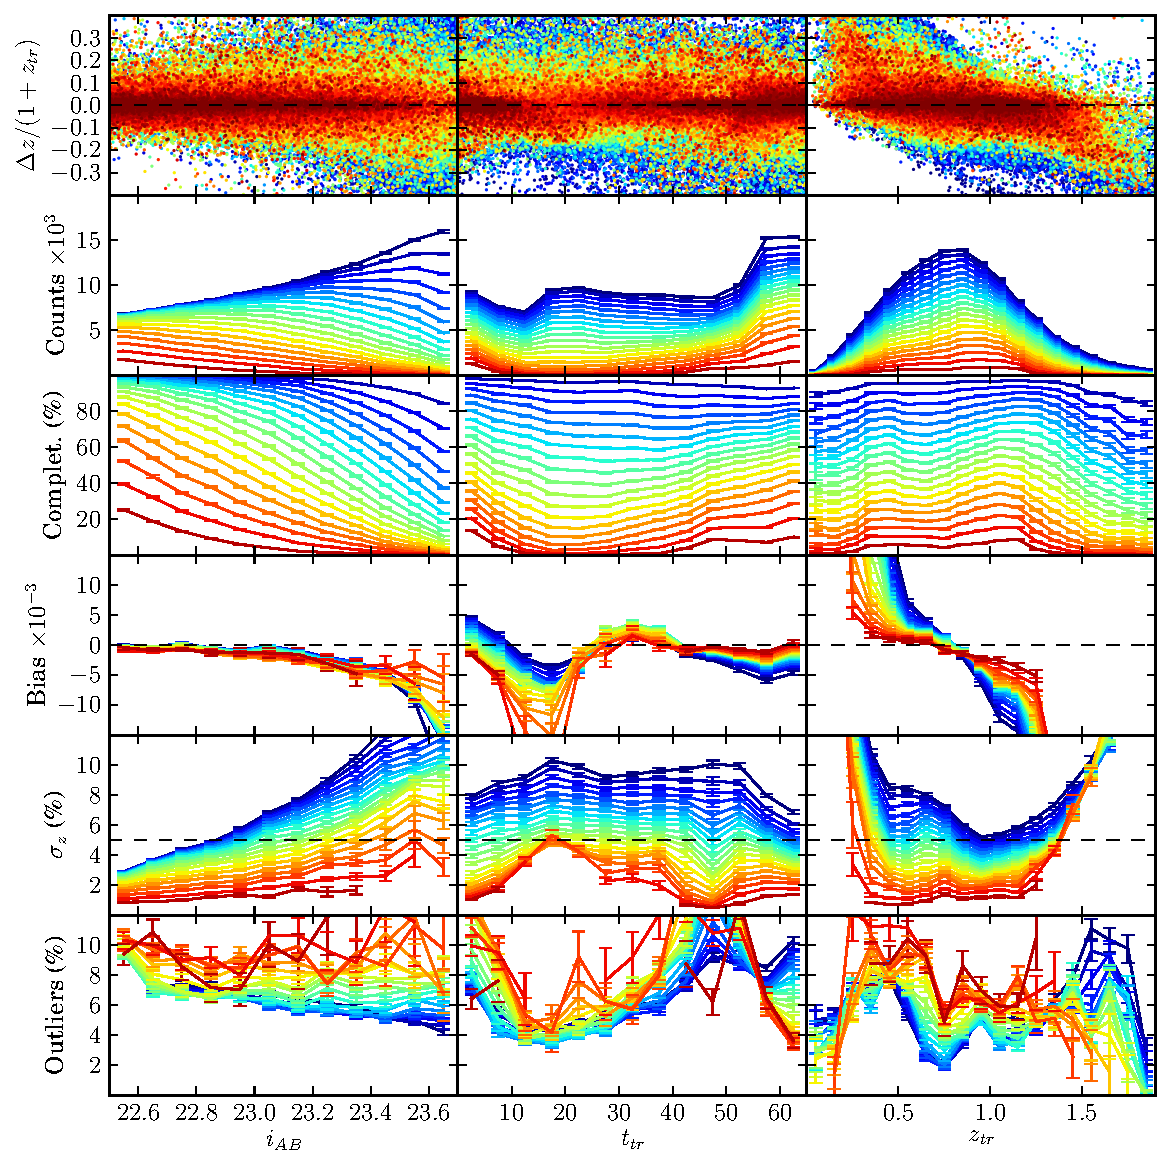
\includegraphics[type=jpg,ext=.jpg,read=.jpg, width=130mm]{./plots/mock.r260.n1e6.s10.121027_default_faint}
\caption{Statistics showing the PAU-FS photo-$z$ performance in the same layout as in Fig.~\ref{bs_pz_results}.}
\label{fs_pz_results}
\end{figure*}

\subsection{Narrow bands vs. Broad bands}
We want to quantify the improvement that the NB bring to the photo-$z$ performance. For this purpose, we run \texttt{BPZ} on the BS and the FS using the NB and the BB separately. Then, in Fig.~\ref{Dz_pau_only_BB} and Table~\ref{tab:usefulness_NB}, we compare the results between these runs and also with the original ones when the BB and the NB are used together (BB+NB). Figure~\ref{Dz_pau_only_BB} shows normalized $\Delta z/(1+z_{tr})$ distributions for the BS (red) and the FS (blue) using only the BB (dashed), only the NB (dotted) and both together BB+NB (solid). We see that the resulting distributions when using only BB (dashed) show overall shapes close to Gaussian with perhaps larger tails on both sides. However, when the NB are also included (solid) the peaks of the distributions become clearly sharper. This is more noticeable in the BS than in the FS, because the non-observed condition ($\sigma_m<0.5$) defined in Section~\ref{sec:mock} implies that most of the NB are not used in the photo-$z$ determination for the FS. Table~\ref{tab:usefulness_NB} shows bias (median), $\sigma_z$ ($\sigma_{68}$) and $3\sigma$-outlier fraction of each distribution. $\sigma_z$ in the BS is reduced $\sim$4.8 times going from $\sim$3.34\% to $\sim$0.7\% when the NB are included, while the improvement is much less significant in the FS. We also see that bias is reduced by an order of magnitude when the NB are included in both samples. On the contrary, the outlier fraction increases, but as mentioned, this is due to the fact that improvements on $\sigma_z$ penalize the outlier fraction. On the other hand, we see that using NB alone slightly degrades all metrics in the BS and the FS, except the outlier fraction in the FS which is improved for the same reason. In fact, $\sigma_z$ in the FS gets almost twice worse than when only using BB or BB+NB. It seems that in the FS NB by themselves only help the bias, while if they are used together with the BB, the improvement also extends to $\sigma_z$.
\begin{figure}
\centering
\includegraphics[height=84mm]{./plots/Dz_pau_only_BB.pdf}
\caption{Normalized $\Delta z/(1+z_{tr})$ distributions for the BS (red) and the FS (blue) using only BB (dashed), only NB (dotted) or both together BB+NB (solid). Bias, $\sigma_z$ and 3$\sigma$-outlier fraction of each distribution are shown in Table~\ref{tab:usefulness_NB}.}
\label{Dz_pau_only_BB}
\end{figure}

\begin{table}
\centering
\begin{tabular}{cccccccc}
\cline{2-4}
 & \multicolumn{3}{c}{Bright Sample} \\
\cline{2-4}
 & BB & NB & BB + NB \\
\cline{1-4}
\multicolumn{1}{c}{Bias$\times10^{-4}$} & -31.64 & -3.31 & -2.18 \\
\multicolumn{1}{c}{$\sigma_z$(\%)} & 3.34 & 0.83 & 0.70 \\
\multicolumn{1}{c}{Outliers(\%)} & 4.41 & 18.19 & 13.28 \\
\cline{1-4}
 & \multicolumn{3}{c}{Faint Sample} \\
\cline{2-4}
 & BB & NB & BB + NB \\
\cline{1-4}
\multicolumn{1}{c}{Bias$\times10^{-4}$} & -152.66 & -41.19 & -19.01 \\
\multicolumn{1}{c}{$\sigma_z$(\%)} & 9.38 & 16.17 & 8.86 \\
\multicolumn{1}{c}{Outliers(\%)} & 6.79 & 4.90 & 7.18 \\
\cline{1-4}
\end{tabular}
\caption{Bias (median), $\sigma_z$ ($\sigma_{68}$) and $3\sigma$-outlier fraction when using only BB, only NB or both together BB+NB for the bright and faint samples.}
\label{tab:usefulness_NB}
\end{table}


\subsection{Impact of the photo-$z$s on clustering}
We want to study the impact of the PAU photo-$z$ performance on the measurements of angular clustering. In \citet{Gaztanaga2012} it is shown that galaxy cross-correlation measurements $\bar{\omega}_{ij}$ between two photo-$z$ bins $i$ and $j$ are related to their cross-correlation between real redshift bins $\omega_{ij}$ as
\begin{equation}
\bar{\omega}^{A\times B}_{ij} = \sum_{kl} r^A_{ik} \omega^{A \times B}_{kl} r^B_{jl} = r_A \cdot \omega^{A \times B} \cdot  r^T_B,
\label{eq:wijbar}
\end{equation}
where $r_{ij}$ is called the migration matrix and gives the probability that a galaxy observed at the photo-$z$ bin $i$ will be actually at the true redshift bin $j$, while $A$ and $B$ denote different galaxy samples. We compute the migration matrices from the PAU photo-$z$ simulations and show them on Fig.~\ref{plot:rij} for the BS (top) and the FS (bottom) in photo-$z$ bins of width $0.014(1+z)$, which is four times the photo-$z$ precision $\sigma_z$ in the BS once the photo-$z$ quality cut that leaves a 50\% completeness is applied. Note that the matrices are normalized row-wise by definition. The FS migration matrix has quite a  thick diagonal, i.e. around $z_{tr} \simeq 1$ the width is $\Delta z \simeq 0.1$ for $\simeq 10\%$ probabilities and $\Delta z \simeq 0.4$ for $\simeq 1\%$. There are also outliers going from very large true redshifts 
$z_{tr} \simeq 1.8$ to lower photo-$z$ redshifts and some from low true redshifts up to  $z_{ph} \simeq 1$. The  BS has a 
thinner diagonal with $\Delta z < 0.04$ at $\simeq 1\%$ probability and with fewer outliers.
These values are of course in agreement with previous results in Figs.~\ref{dz_hist} and \ref{pz_results}.

\begin{figure}
\centering
\includegraphics[width=84mm]{./plots/rij_pau.pdf}
\caption{The resulting migration matrices $r_{ij}$ from the PAU photo-$z$ simulations after applying the photo-$z$ quality cut that leaves 50\% completeness. The top plot corresponds to the BS and the bottom plot to the FS. For a higher contrast and clarity we plot the logarithm of the matrix values. These matrices give the probability that a galaxy observed at the photo-$z$ bin $i$, will be actually at the true redshift bin $j$. The bin widths are $0.014(1+z)$, four times the photo-$z$ precision expected in the BS.}
\label{plot:rij}
\end{figure}

\begin{figure*}
\centering
\makebox[0cm]{\includegraphics[width=170mm]{./plots/wij_pau.pdf}}
\caption{Top panels show the angular auto (diagonal) and cross- (off-diagonal) correlations $\omega_{ij}$ at 1~arcmin between the true redshift bins $i$ and $j$ of the BS (left), the FS (middle) and the crossing of both of them (right). Bottom plots show the same correlations but measured with photo-$z$ bins, which can be computed by using Eq. (\ref{eq:wijbar}) with the migration matrices in Fig.~\ref{plot:rij}. The bin widths are $0.014(1+z)$, four times the photo-$z$ precision expected in the Bright Sample.}
\label{plot:wij}
\end{figure*}

To illustrate how these matrices affect angular clustering measurements, we use a simple model to
predict $\omega_{ij}$ at an arbitrary reference angular scale, $\theta$, of 1~arcmin. We include intrinsic
galaxy clustering and weak lensing magnification:
\begin{eqnarray}
\label{eq:all4}
w_{ij} &=& w_{G_iG_j}+ w_{G_i\mu_j} + w_{\mu_i  G_j}+ w_{\mu_i\mu_j} \\
w_{G_iG_j} &=&  b_ib_j \int dz_1dz_2  \, \, \phi_{G_i}(z_1) \, \phi_{G_j}(z_2)  \, \, \xi(r_{12}) \\
 w_{G_i\mu_j} & =&   b_i \alpha_j \int dz_1 dz_2 \, \,\phi_{G_i}(z_1) \, p_{\mu_j}(z_2) \, \, \xi(r_{12}) \\
w_{\mu_i\mu_j} & =&   \alpha_i \alpha_j \int dz_1 dz_2 \,  \, p_{\mu_i}(z_1) \, p_{\mu_j}(z_2) \, \, \xi(r_{12}) 
\end{eqnarray}
where $\xi(r_{12})$ is the non-linear matter 2-point correlation 
between the positions of two galaxies separated in 3D space by $r_{12}=r_2-r_1$, 
where the angular separation between $r_1$ and $r_2$ is fixed to be the reference angle (i.e. $\theta=1$ arcmin),
while the radial separation is integrated out via $z_1$ and $z_2$. We have that
$\phi_{G_i}(z)$ is a top-hat distribution for galaxies in the  redshift bin $i$  and $p_{\mu_j}(z)$ is the efficiency of weak
lensing effect for lenses at $z$ and sources at $z_j$ (following the notation in \citet{Gaztanaga2012}). 
The coefficient $b_i$ is the effective galaxy bias at $z_i$  and 
 $\alpha_j\equiv 2.5s_j-1$ is the amplitude of the weak lensing magnification effect (with $s_j$ the slope
of the galaxy number counts at the flux limit of the sample at $z_j$). 
The first equation above has 4 terms corresponding to galaxy-galaxy
(intrinsic clustering), galaxy-magnification, magnification-galaxy  and 
magnification-magnification correlations. In our test, we use $\alpha_i=1$ and $b_i=1$
to generate the starting point for $\omega_{ij}$. We then apply
the following transformation:
\begin{eqnarray}
\omega^{B\times B}_{ij} \rightarrow b_{B}(z_i)b_{B}(z_j)\omega_{ij} \\
\omega^{F\times F}_{ij} \rightarrow b_{F}(z_i)b_{F}(z_j)\omega_{ij} \\
\omega^{B\times F}_{ij} \rightarrow b_{B}(z_i)b_{F}(z_j)\omega_{ij}
\end{eqnarray}
depending on which galaxy samples we are cross-correlating (FS or BS), where
\begin{eqnarray}
b_{B}(z_i) &=& 2 + 2 (z_i - 0.5) \\
b_{F}(z_i) &=& 1.2 + 0.4 (z_i - 0.5)
\end{eqnarray}
are the biases in the BS and FS respectively in the photo-$z$ bin $i$ (at mean redshift $z_i$). This corresponds
to using linear bias for the intrinsic  correlation (as in \citet{Gaztanaga2012}) and some particular evolving
slope ($s_i \sim 1$) for the magnification cross-correlations.
 In Fig.~\ref{plot:wij} we show $\omega^{B\times B}_{ij}$ (left), $\omega^{F\times F}_{ij}$ (middle) and $\omega^{B\times F}_{ij}$ (right) before (top) and after (bottom) being transformed by the migration matrices $r_{ij}$ in Fig.~\ref{plot:rij} through Eq. (\ref{eq:wijbar}). Note that for the $B\times B$ and $F \times F$ cases the correlations matrices are symmetrical. Also note that the redshift ranges in both samples are different, so that the $B \times F$ correlation matrix is not squared.

 In the top panels, we can see the
intrinsic galaxy-galaxy clustering in the diagonal of the matrix, which has an amplitude of order unity and
decreases rapidly to zero for separated redshift bins. 
The galaxy-magnification correlation appears as a diffused off-diagonal cloud with an 
amplitude $<0.05$ (clear colors). The magnification-magnification contribution is negligible.
In the bottom panel, we see the effect of the photo-$z$ migration. The diagonal
(auto-correlations) becomes thicker and diluted. The off-diagonal galaxy-magnification cloud becomes
 more diffused, especially for the FS. The cross-correlation $F \times B$ produces results that are intermediate
between $B \times B$ and $F \times F$.

We can invert the migration matrices to go from the bottom
panels (which are the observations $\bar{\omega}^{A\times B}$) to the top panels (i.e. true correlations
$\omega^{A \times B}$) by inverting Eq. (\ref{eq:wijbar}):

\begin{equation}
 \omega^{A \times B} = r_A^{-1} \cdot \bar{\omega}^{A\times B}  \cdot  (r^T_B)^{-1} 
\label{eq:wij}
\end{equation}
This should work perfectly well if we can calibrate the $r_{ij}$ matrices properly. For a large
fiducial survey with about 5000 sq. deg. we need about $\simeq 1\%$ accuracy in $r_{ij}$
\citep{Gaztanaga2012}. In practice, the accuracy of the above reconstruction
 can be used to put requirements on the photo-$z$ calibration.
